 \section{Deeper Issues}
In a first reading you can skip the next sections that present some finer aspects of message identification.

\subsection{Deeper into Parenthesis}
Knowing that the message \ct{+} when sent to a point with a point returns a point representing the sum of the two points we let you follow the way binary messages are executed in the expression \ct{(50@60) + (200@400)} which returns the point \ct{250@460} as illustrated in Figure~\ref{fig:compoBinBracket}. Now if you want to understand the result returned by the expression \ct{50@60 + 200@400} illustrated in Figure~\ref{fig:compoBinNoBracket}, read \tcharef{ch:absoluteLocation} which presents points.


\begin{figure}[h]
\centerline{
\includegraphics[width=5cm]{ucompoBinBracket}} 
\caption{Another example of using parentheses to control the way messages are executed.\label{fig:compoBinBracket}}
\end{figure}

\begin{figure}[h]
\centerline{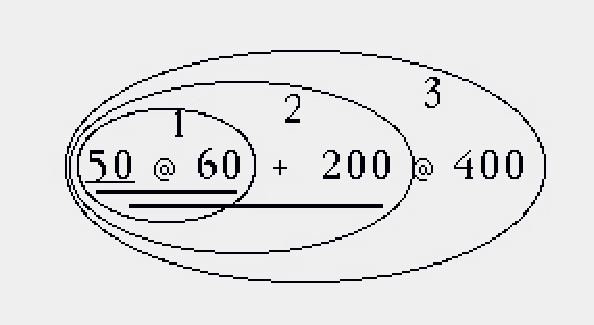
\includegraphics[width=5cm]{ucompoBinNoBracket}} 
\caption{As the message \ct{@} when sent to a \textit{point} returns a B3DVector, the expression does not return a simple point but a B3DPoint.  \label{fig:compoBinNoBracket}}
\end{figure}




Note that evaluating from left to right and the other rules we explained is equivalent to put around parentheses. Here are some expressions without and their equivalent with parentheses. Note that you do not have to really understand what these expressions are meaning, you just have to identify the different kinds of messages.

\begin{scriptwithtitle}{Expressions and their equivalence fully parenthesized}
Turtle new east 
    (Turtle new) east

100@200 = 200@300
	((100@200) = 200) @ 300
	
20 + 2 * 5 + 2
   ((20 + 2) * 5) + 2

5 between: 1 and: 3 squared + 4
   5 between: 1 and: ((3 squared) + 4)

2 factorial + 4
    (2 factorial) + 4
\end{scriptwithtitle}



\subsection{Identifying Complex Keyword-based Messages}

As we already mentioned, messages can have multiple arguments. In such a case, keyword-based messages are used. A keyword-based message can be composed of several words terminated by the character \ct{:}. In \tscrref{scr:longkey} the message \ct{between:and:} is sent to 1. This message can be written on two different lines without problem. This message contains two \ct{:} so it requires two arguments. In fact a keyword-based message is the longest sequence of words terminated by \ct{:} that is not interrupted by the characters \ct{.} or \ct{;}.

\begin{scriptwithtitle}{Examples of long keyword based messages}\label{scr:longkey}
1 \textbf{between:} 5 \textbf{and:} 10.

1 \textbf{between:} 5 
  \textbf{and:} 10.
\end{scriptwithtitle}

In fact this is a bit more complex. The characters \ct{[}, \ct{]}, and \ct{(}, \ct{)} delimit distinct areas. In such an area, a keyword-based message is the longest sequence  of words terminated by \ct{:} that is not cut by the characters \ct{.},  or \ct{;}.  \Tscrref{scr:keywordComplex} illustrates this point.
We use different style (italic, bold...) to group together the words belonging to a same keyword-based message.

\begin{scriptwithtitle}{Identifying keyword-based messages}\label{scr:keywordComplex}
1   | dist| 
2   dist := self \textit{distanceBetween:} (World bounds \textbf{centeredBy:} self topLeft)
3                \textit{and:} self position.
4   dist > 300
5      \textbf{ifTrue:} [self \textit{color:} Color green \textit{withSize:} 2]
6      \textbf{ifFalse:} [dist < 200
7         ifTrue: [self \textit{color:} Color red]
8         ifFalse: [self \textit{color:} Color yellow]]
\end{scriptwithtitle}

\Tscrref{scr:keywordComplex} can be seen as \tscrref{scr:keywordComplex2} where we replaced the first level areas by \ct{xxx}. 

\begin{scriptwithtitle}{Identifying keyword-based messages}\label{scr:keywordComplex2}
1   | dist| 
2   dist := self \textit{distanceBetween:} xxx
3                \textit{and:} self position.
4   dist > 300
5      \textbf{ifTrue:} xxx
6      \textbf{ifFalse:} [dist < 200
7         ifTrue: xxx
8         ifFalse: xxx]
\end{scriptwithtitle}

\begin{itemize}
\item Line 2 contains \ct{(World bounds centeredBy: self topLeft)} which creates a distinct area. In such an area there is one complete keyword-based message \ct{centeredBy:}. 

\item Line 2 contains the word \ct{distanceBetween:}. It does not represent a complete keyword-based message because there is not \ct{.} or \ct{;} so we pass to the next line. Note that the word \ct{centeredBy:} does not participate in the keyword-based message starting with \ct{distanceBetween:} because it is in a distinct area delimited by \ct{(} and \ct{)}.

\item The line 3 complements the keyword-based message with  the word \ct{and:}. There is a dot at the end so the message is finally \ct{distanceBetween:and:}. 

\item Line 5 contains \ct{[self color: Color green withSize: 2]} which creates another distinct area. In such an area, there is the keyword-based message \ct{color:withSize:}. 

\item Lines 7 and 8 defines two distinct areas that contain the same keyword-based message \ct{color:}. 

\item Lines 6, 7 and 8 define one extra area \ct{[dist < 200 ifTrue: [self color: Color red]  ifFalse: [self color: Color yellow]]} containing the two smaller areas identified above. This bigger area contains the message \ct{ifTrue:ifFalse:} starting at line 7.

\item Lines 5, 6, 7 and 8 contain the message \ct{ifTrue:ifFalse:}. This message is sent to the result of the message \ct{dist>300} on line 4.
\end{itemize}

\begin{largecadre}{
The characters \ct{[}, \ct{]}, and \ct{(}, \ct{)} delimit distinct areas. In such an area, 
a keyword-based message is the longest sequence  of words terminated by \ct{:} that is not cut by the characters \ct{.},  or \ct{;}. 
When the characters \ct{[}, \ct{]}, and \ct{(}, \ct{)} surround some words, these words participate in the keyword-based message local to the area defined.}
\end{largecadre}


The problem is that when we compose two keyword-based messages sometimes we want to say
that the message is \textit{not} the longuest sequence of words. For example in \tscrref{scr:withParenthesis2}  we want to send a rectangle the message \ct{containsPoint:} and not \ct{containsPoint:ifTrue:} which does not exist. For this reason we put parenthesis around the message \ct{aRect \textbf{containsPoint:} aTurtle center}. This creates a new area and distinguish the message \ct{containsPoint:} and \ct{ifTrue:} as two complete keyword-based messages. 

\begin{scriptwithtitle}{Conditional Requiring Parenthesis}\label{scr:withParenthesis2}
| aRect aTurtle |
aTurtle := Turtle new.
aRect := Rectangle origin: 100@200 corner: 300@400.
\textbf{(}aRect \textbf{containsPoint:} aTurtle center\textbf{)}
    \textbf{ifTrue:} [Smalltalk beep]
\end{scriptwithtitle}


\largecadre{Use \ct{(} and \ct{)} to disambiguate two keyword-based message.}



%\subsection{A Final Note}

%Binary messages are not limited to manipulate numbers. \Tscrref{scr:binary2} shows some other examples of binary messages. We see clearly that the same messages that have been sent to numbers are now sent to other objects. This practice will be explained in \charef{cha:polymorphism}. In short, the same message can be sent to different kind of objects such as number, string, as soon as it make sense for them. Each kind of object will execute the message according to its own way of doing things. For example, we can add to number by sending the message \ct{+} to a number and it returns the number sum. Similarly we can send the message \ct{+} to a point with another point and it will return the sum. Even though the sum of number and point are different operations. 

%
%\begin{scriptwithtitle}{Examples of Binary Messages on Various Objects}\label{scr:binary2}
%'aaaa' \textbf{>} 'aaab'   "Comparing strings (sequence of characters)"
%\pr false 
%'stephane' \textbf{=} 'stephanee'  "Equality between two strings (sequences of characters)"
%\pr false
%'stephane' \textbf{~=} 'stephanee'    "Difference between two strings"
%\pr true
%caro direction \textbf{=} 0                   "Equality"
%\pr true
%(caro direction = 0) \textbf{|} (caro direction = 90)                 "Or between two booleans"
%\pr true 

%(caro direction = 0) \textbf{&} (caro penSize = 2)                   "And between two booleans"
%\pr true
%\end{scriptwithtitle}


